\documentclass{beamer}
\usepackage[latin1]{inputenc}
\usepackage[french]{babel}
\usepackage{graphicx}
\usepackage{color}
\usepackage{colortbl}
\usepackage{tabularx}
\usepackage{tikz}
\setbeamertemplate{blocks}[rounded][shadow=true]
\usetheme{Warsaw}
\usecolortheme{orchid}
\title[Soutenance stage ing�nieur \hfill 29/08/2013]{Soutenance stage ing�nieur}
\author{Yicheng GAO}
\date{29 ao�t 2013}
\institute{INSA de Rouen}
\addtobeamertemplate{footline}{\hfill\insertframenumber/\inserttotalframenumber\hspace{2em}\null}
% 30 mins de pr�sentation

% --------------------- --------------------- --------------------- --------------------- --------------------- %

\AtBeginSection[]{
  \begin{frame}{Sommaire}
  \small \tableofcontents[currentsection, hideothersubsections]
  \end{frame} 
}

\begin{document}

\definecolor{bleu}{rgb}{0.20,0.20,0.82}
\definecolor{vert}{rgb}{0.16,0.85,0.20}

% ------------ PAGE DE GARDE-------------- %

\begin{frame} 
  	\titlepage
	\begin{center}
	Tuteur INSA: Abdelaziz Bensrhair\\
	Tuteur entreprise: Jean-Philippe AUTHIER
	\end{center}

	\begin{center}
		\begin{minipage}[c]{10cm}
			\begin{center}
				
\includegraphics[width=3cm]{images/logoasi}
				
\includegraphics[width=3cm]{images/UINTWhiteBackGround}
			\end{center}
		\end{minipage}
	\end{center}
\end{frame}

% --------------- PLAN ----------------- %

\begin{frame} 
	\frametitle{Le Plan}
	\tableofcontents[hidesubsections]{}
\end{frame}

% ----------- INTRODUCTION -------------- %
\section{Introduction}
\begin{frame}
\frametitle{Introduction}
	\begin{block}{Stage ing�nieur}
		\begin{itemize}
		\item Stage ing�nieur de 25/03/2013 � 31/08/2013 
		\item Stage en commun avec Master 2 SSI d'universit� de Rouen
		\item Chez soci�t� UINT situ� � SAINT AUBIN (91)
		\item Tuteur INSA: Abdelaziz Bensrhair
		\item Tuteur entreprise: Jean-Philippe AUTHIER (Directeur logiciel R\&D)
		\end{itemize}
	\end{block}

	\begin{exampleblock}{Sujet du stage}
	L'optimisation d'un syst�me d'authentification forte dont le mot de passe dynamique est g�n�r� en acoustique \hfill (\textbf{Carte acoustique})
	\end{exampleblock}
\end{frame}


\section{Pr�sentation de l'entreprise}
% ? mins environs

% ------------------------- %
\begin{frame}
\frametitle{Pr�sentation de l'entreprise (1/4)}
	\begin{block}{UINT}
	\begin{itemize}
	\item Fond�e en Avril 2008. UINT veut �tre reconnue comme une soci�t� tr�s innovante, pionni�re et leader dans le domaine des cartes � �nergie embarqu�e.
	\item R�compens�e �Jeune Entreprise Innovante�
	\item Prix de la �Start-UP de l'ann�e 2010� d�cern� par ElectroniqueS
	\item Prix de �l'innovation internationale 2010� d�cern� par la CCIE et la CGPME 91
	\item Equipe compos�e de 8 ing�nieurs/docteurs reconnus pour leur expertise dans le domaine des cartes �lectroniques (�Oscard de la meilleure technologie dans une carte bancaire�) et (�Finaliste 2009 des SESAMES AWARDS Cartes 2009�).
	\end{itemize}	
	\end{block}
	\end{frame}


% ------------------------- %
\begin{frame}
\frametitle{Pr�sentation de l'entreprise (2/4)}

	\begin{block}{Power Inlay Technologies}
	\begin{itemize}
	\item UINT Card Platform
		\begin{itemize}
		\item ISO 7810
		\item Process de lamination � froid, ti�de ou chaud
		\end{itemize}
	\item D�veloppement de firmware
	\end{itemize}
	\end{block}
	\begin{figure}
	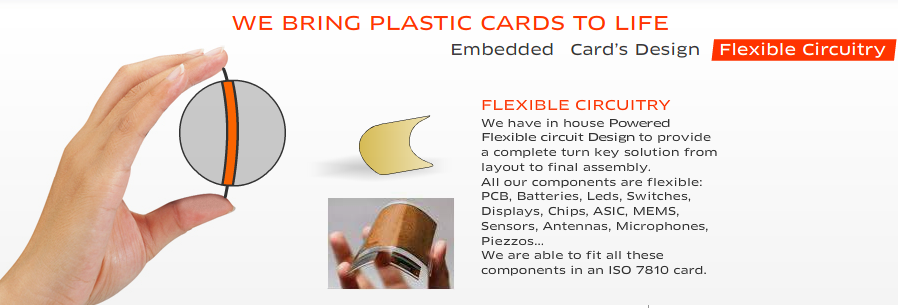
\includegraphics[width=\textwidth]{images/flx}	
	\end{figure}
\end{frame}

% ------------------------- %
\begin{frame}
\frametitle{Pr�sentation de l'entreprise (3/4)}
	\centering
	Domaines: S�curit�, sant�, jeu, marketing
	\begin{figure}
	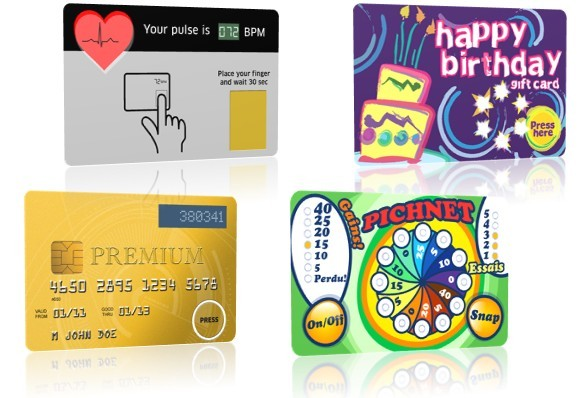
\includegraphics[scale = 0.6]{images/carte.jpg}	
	\end{figure}
\end{frame}

% ------------------------- %
\begin{frame}
\frametitle{Pr�sentation de l'entreprise (4/4)}
\framesubtitle{Projet Carte acoustique}
	\begin{figure}
	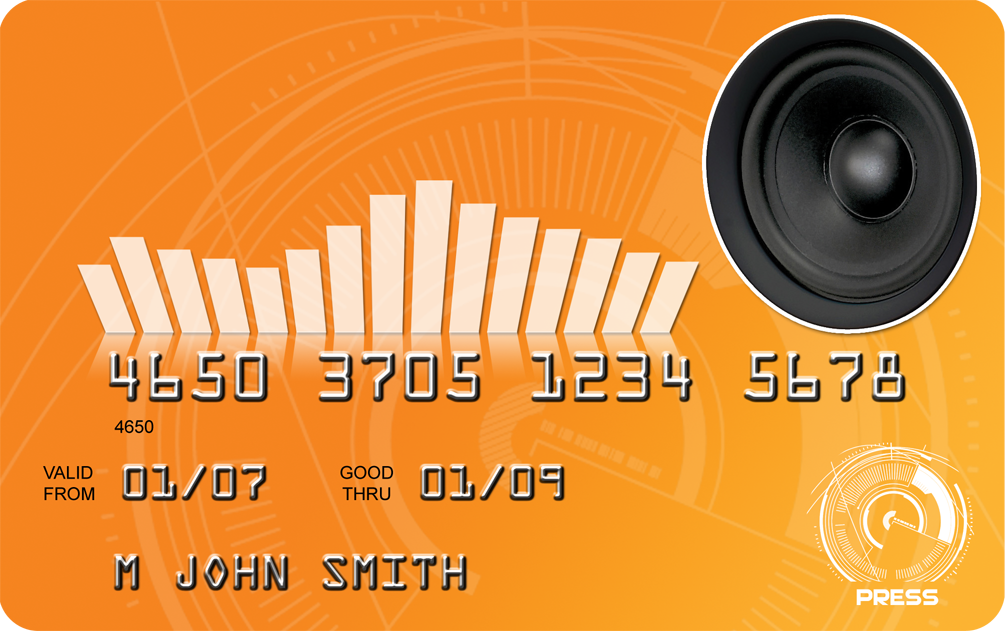
\includegraphics[scale = 0.225]{images/carteavant}	
	\caption{Face avant d'une carte acoustique}
	\end{figure}
	\begin{block}{Fonctionnalit�s g�n�rales}
La carte acoustique �met une s�quence acoustique unique � chaque pression du bouton. La carte utilise un microprocesseur pour calculer les deux OTP (One Time Password). L'�nergie utilis�e provient d'une batterie fine et flexible.
	\end{block}
\end{frame}



% ---------- CORPS DU PROJET ------------ %
\section{Contexte de travail}
% ? mins environs

% ------------------------- %

\begin{frame}
\frametitle{Contexte de travail (1/4)}
\framesubtitle{Caract�ristiques g�n�rales de la carte acoustique}
	\begin{figure}
	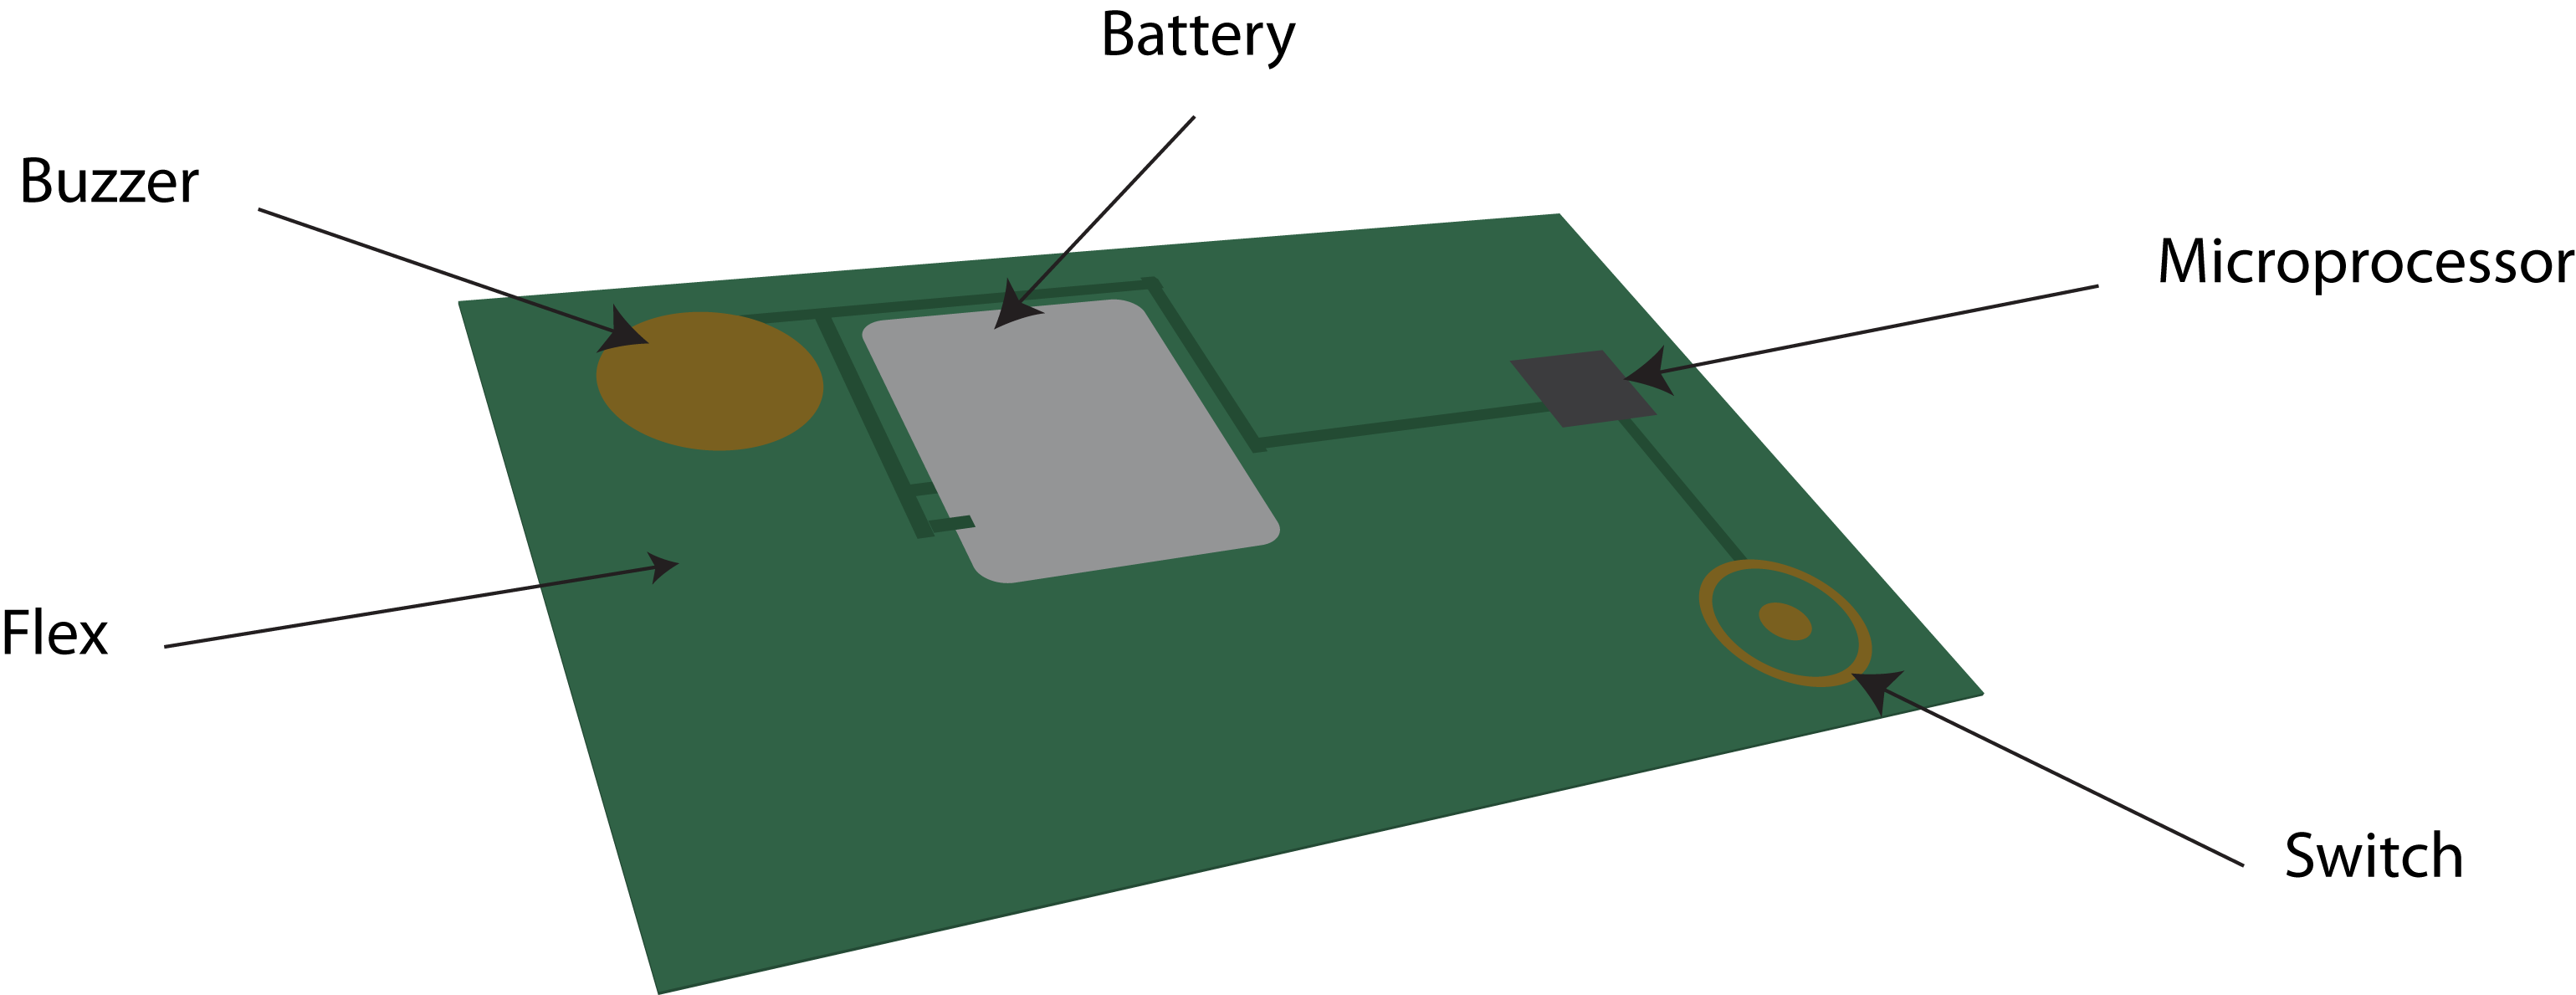
\includegraphics[scale = 0.3]{images/carteinside}	
	%\caption{Sch�ma d'une carte acoustique}
	\end{figure}

	\begin{block}{L'�lectronique embarqu�e est compos�e des �l�ments}
	\begin{itemize}
	\item Int�gr�s sur un circuit imprim� flexible, ou � flex �
	\item Soud�s au � flex � par un processus de capillarit�
	\item Flex composants est appel� Inlay
	\item Int�gr� � l'int�rieur de la carte PVC
	\end{itemize}
	\end{block}
\end{frame}

% ------------------------- %
\begin{frame}
\frametitle{Contexte de travail (2/4)}
\framesubtitle{Caract�ristiques g�n�rales de la carte acoustique}
\centering
Organigramme de fonctionnement de la carte acoustique
	\begin{figure}
	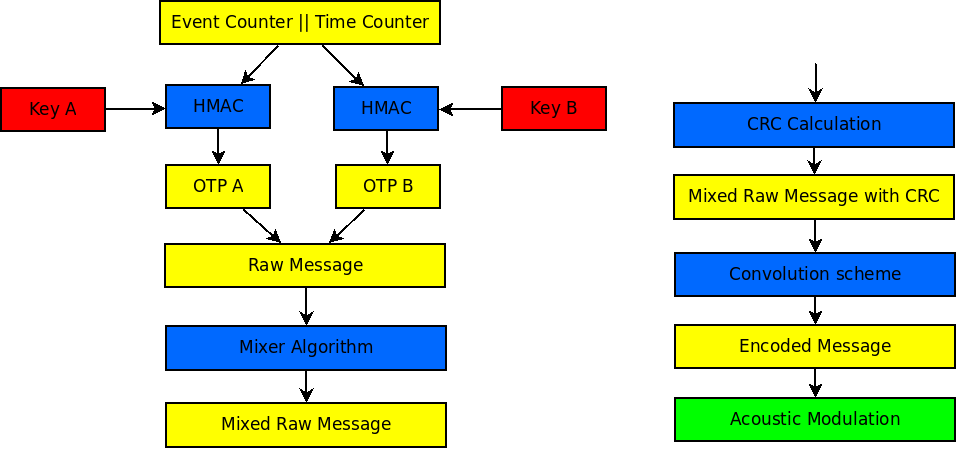
\includegraphics[scale = 0.3]{images/organigramme2}	
	\caption{Fonctionnement de la carte acoustique}
	\end{figure}
\end{frame}

% ------------------------- %
\begin{frame}%[plain]
\frametitle{Contexte de travail (3/4)}
\framesubtitle{Caract�ristiques g�n�rales de la carte acoustique}
	\begin{block}{Les constantes et variables essentielles}
	\begin{itemize}
	\item Les cl�s cryptographiques (HOTP KeyA \& HOTP KeyB) 
	\item Le compteur d'�v�nements (Event Counter) 
	\item Le num�ro de s�rie (Id)
	\end{itemize}
	\end{block}

	\begin{exampleblock}{G�n�ration du cryptogramme acoustique}
	\begin{itemize}
	\item La g�n�ration d'un HOTP et du cryptogramme
	\item L'encodage du cryptogramme 
	\begin{itemize}
		\item Le cryptogramme et les symboles
		\item Le m�langeur
		\item L'ajout du CRC16 au message 
		\item Le codage convolutif 
	\end{itemize}
	\item La restitution du cryptogramme 
	\end{itemize}
	\end{exampleblock}

\end{frame}


% ------------------------- %
\begin{frame}
\frametitle{Contexte de travail (4/4)}
\framesubtitle{Caract�ristiques g�n�rales de la carte acoustique}
	\begin{block}{Les trois versions}
	\begin{itemize}
	\item \textbf{V4G}
	\item V0 
	\item V1
	\end{itemize}
	\end{block}

	\begin{exampleblock}{Les outils}
	\begin{itemize}
	\item Offline: L'utilitaire \textit{ListenAcousticMessage\_V1.2.1.35.exe}
	\item Online: \href{http://solution.uint.info/Acoustictechno/}{La page de test}
	\item Authentification (SAS)
	\end{itemize}
	\end{exampleblock}
\end{frame}




\section{Le travail effectu�}
\begin{frame}
\frametitle{Le travail effectu�}
	\begin{block}{Deux parties}
	\begin{itemize}
	\item Plate-forme de tests
	\item Plate-forme de d�monstration
	\end{itemize}
	\end{block}
\end{frame}

\subsection{Plate-forme de tests}
\begin{frame}
\frametitle{Le travail effectu�}
\framesubtitle{Plate-forme de tests (1/5)}
	\begin{block}{Objectif}
        �valuer la performance de carte acoustique Version 4G
	\end{block}

	\begin{exampleblock}{Proc�dure}
	\textbf{Phase 1:} Plan du test\\
	\textbf{Phase 2:} D�marrage du test\\
	\textbf{Phase 3:} Analyse des r�sultats
	\end{exampleblock}

\end{frame}

% ------------------------- %
\begin{frame}
\frametitle{Le travail effectu�}
\framesubtitle{Plate-forme de tests (2/5)}

\begin{columns}
\begin{column}[l]{0.6\textwidth}
	\begin{exampleblock}{Plan du test}
\textbf{TEST 1:} Fiabilit� de l'encryptage\\
\textbf{TEST 2:} Fiabilit� �mission sonore\\
\textbf{TEST 3:} Consommation\\
\textbf{TEST 4:} Dur�e de vie\\
\textbf{TEST 5:} R�cup�ration via IPad\\
\textbf{TEST 6:} R�cup�ration via IPhone\\
\textbf{TEST 7:} R�cup�ration via Windows
	\end{exampleblock}
\end{column}
\begin{column}[r]{0.4\textwidth}
	\begin{exampleblock}{Facteurs}
\begin{itemize}
\item Distances
\item Importance
\item P�riph�riques
\item Environnements
\item Versions
\item Phases
\item Nombre de tests
\item Logiciel utilis�
\end{itemize}
	\end{exampleblock}
\end{column}
\end{columns}
\end{frame}

% ------------------------- %
\begin{frame}
\frametitle{Le travail effectu�}
\framesubtitle{Plate-forme de tests (3/5)}
	\begin{figure}
	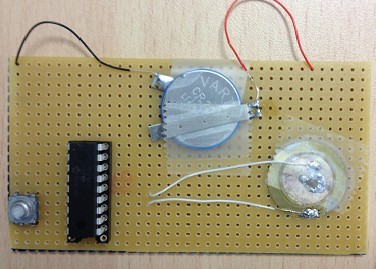
\includegraphics[width=0.5\textwidth]{images/p1}	
	%\caption{Prototype utilis�}
	\end{figure}
\begin{exampleblock}{Strat�gie}
\textbf{Le prototype:} g�n�re une s�quence de 100 messages acoustiques
\end{exampleblock}
\end{frame}

% ------------------------- %
\begin{frame}
\frametitle{Le travail effectu�}
\framesubtitle{Plate-forme de tests (4/5)}

\begin{exampleblock}{Strat�gie}
\textbf{Le prototype:} g�n�re une s�quence de 100 messages acoustiques
\end{exampleblock}

\begin{block}{Environnement du code source}
\begin{itemize}
\item IDE: MPLAB V.8
\item Language: Assembleur
\item Compilateur: MPASM
\item Microcontr�leur: PIC16F648A (Microchip)
\begin{itemize}
\item 256 octets RAM
\item 4096 mots flash
\item communication usart uniquement
\item 1 vecteur interruption
\end{itemize}
\end{itemize}
\end{block}
\end{frame}

% ------------------------- %
\begin{frame}
\frametitle{Le travail effectu�}
\framesubtitle{Plate-forme de tests (5/5)}

\begin{block}{Analyse des r�sultats}
\begin{itemize}
\item Traitement statistique des r�sultats
\item Analyse de l�effet filtrage sous PC
\item Analyse de volume de son par sonom�tre
\item Diff�rences entre les prototypes et les cartes
\item Analyse de l�effet environnement
\end{itemize}
\end{block}
\end{frame}









\subsection{Plate-forme de d�monstration}
\newpage
\section{Plate-forme de démonstration}

Cette section décrit l’utilisation de la carte acoustique dans le contexte d’un achat en ligne.
L’intégration des différents composants technologiques permettant sa réalisation est également détaillée. 

\subsection{Guide d’utilisation}

\textbf{Etape 1: page d’accueil}\\

L’utilisateur arrive sur la page d’accueil d’un site de commerce électronique. Il souhaite acheter cette télévision en promotion. Il clique sur «Add to cart»
\begin{figure}[!htbp]
  \centering
    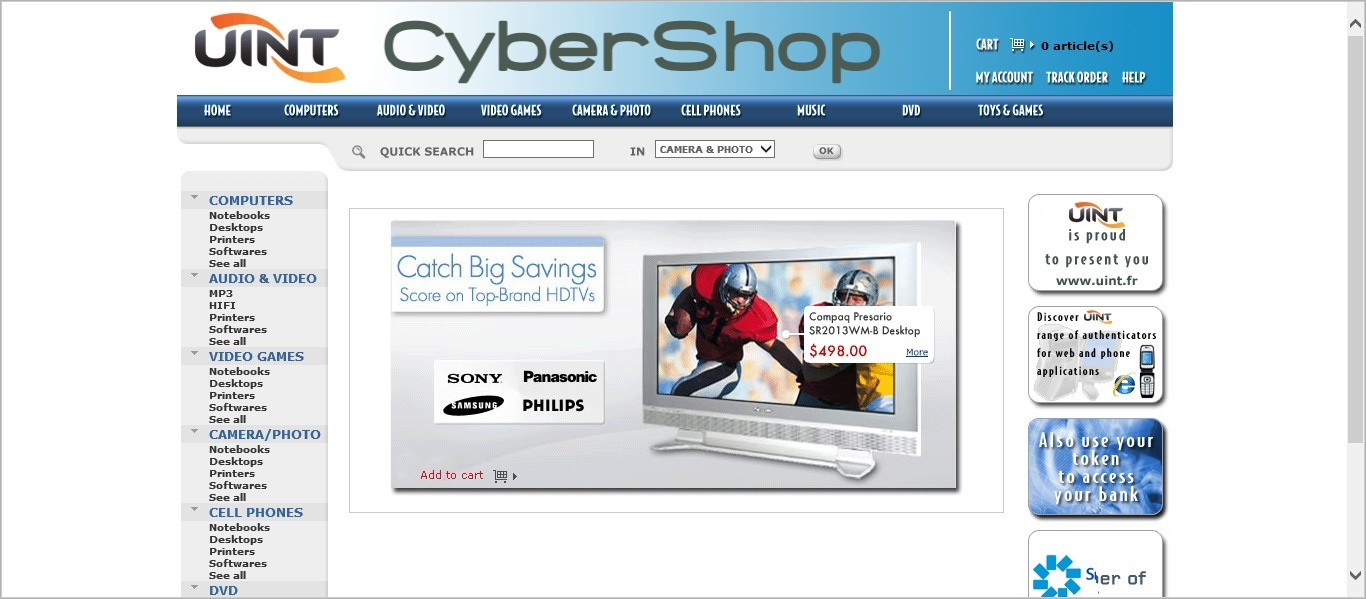
\includegraphics[scale=0.4]{images/1}
  \caption{Etape 1: page d’accueil}
\end{figure}

\textbf{Etape 2: identification}\\

Dans la page suivante, les informations des achats sont visualisés, pour continuer, l’utilisateur est invité à s’identifier.
\begin{figure}[!htbp]
  \centering
    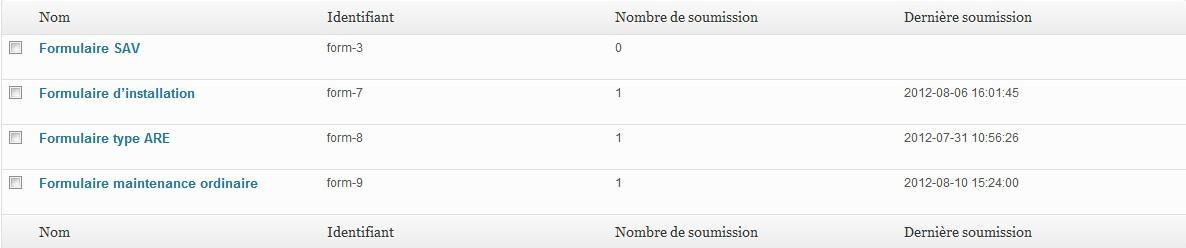
\includegraphics[scale=0.4]{images/2}
  \caption{Etape 2: identification}
\end{figure}

\textbf{Etape 3: choix du mode d’identification}\\

Choix du mode d’identification. L’utilisateur peut choisir d’utiliser sa carte directement dans le navigateur (via l’activeX, étape 4) ou via le serveur vocal.
\begin{figure}[!htbp]
  \centering
    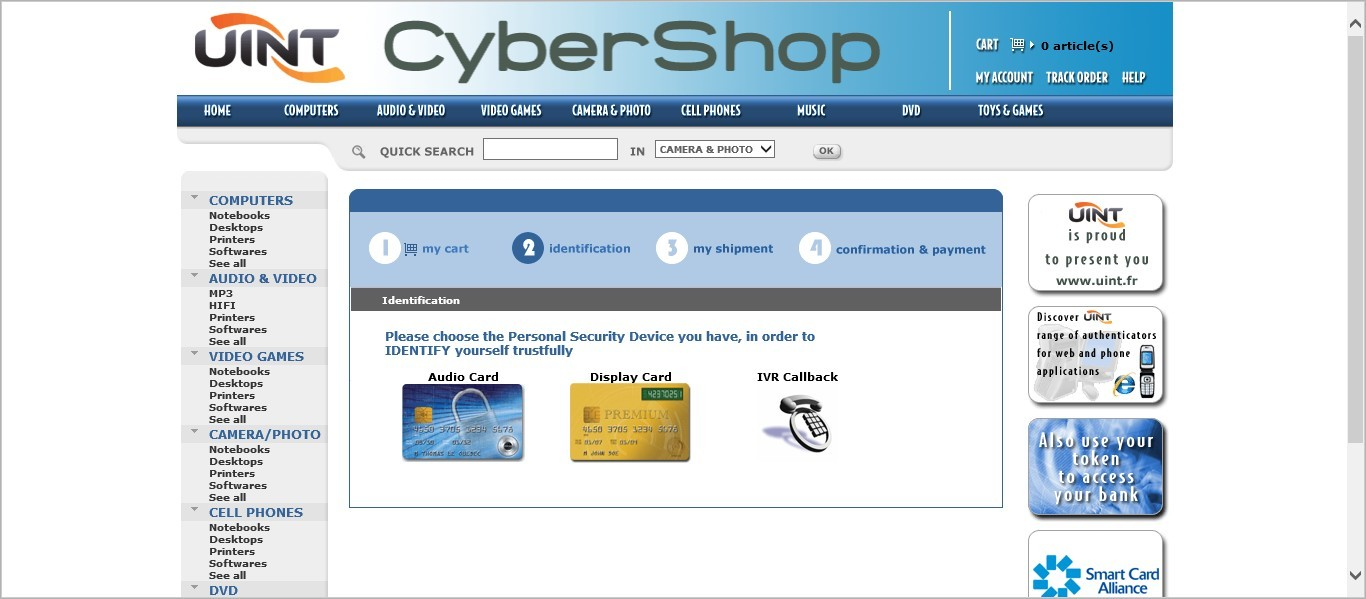
\includegraphics[scale=0.4]{images/3}
  \caption{Etape 3: choix du mode d’identification}
\end{figure}

\vspace{3cm}

\textbf{Etape 4: activeX}\\

En arrivant sur la page d’identification, l’utilisateur s’il arrive pour la première fois sur cette page doit installer un ActiveX. Cet ActiveX, une fois installé, invite l’utilisateur à placer sa carte Wega près du microphone de  son ordinateur et à appuyer sur le bouton de sa carte.
\begin{figure}[!htbp]
  \centering
    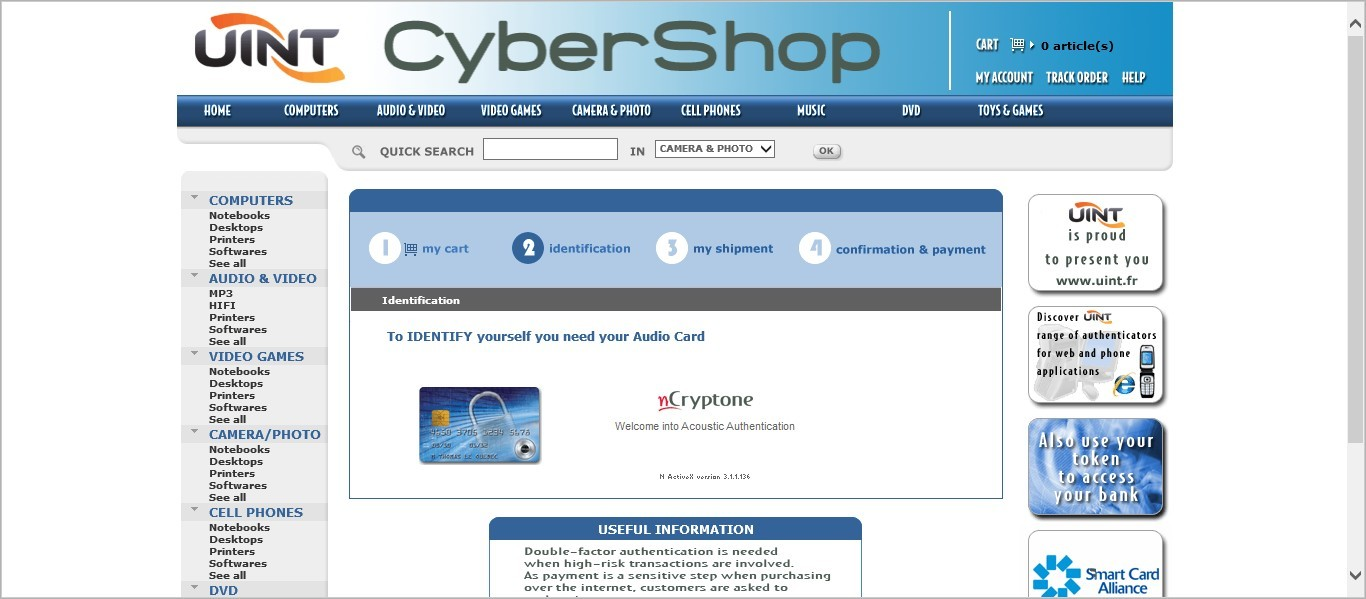
\includegraphics[scale=0.4]{images/4}
  \caption{Etape 4: activeX}
\end{figure}

\newpage
\textbf{Etape 5: livraison}\\

Une fois la carte décodée, le serveur web dialogue avec le serveur d’authentification pour vérifier la validité de la carte. Si la trame acoustique est valide, le serveur d’authentification va alors renvoyer les informations de l’utilisateur qui vont s’afficher dans le navigateur: 
Nom, prénom, adresse,…
\begin{figure}[!htbp]
  \centering
    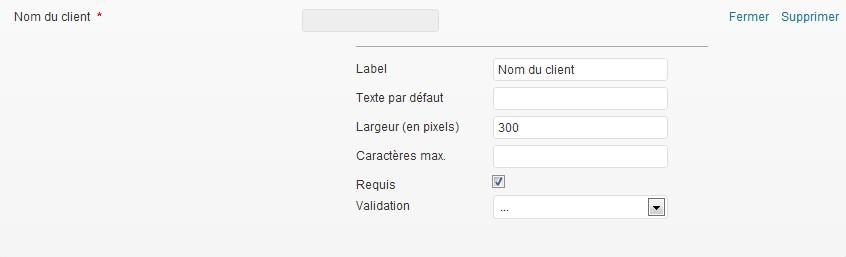
\includegraphics[scale=0.4]{images/5}
  \caption{Etape 5: livraison}
\end{figure}

\vspace{2cm}

\textbf{Etape 6: choix du type de paiement}\\

La prochaine étape est celle du paiement. L’utilisateur est invité à choisir le type de paiement.
\begin{figure}[!htbp]
  \centering
    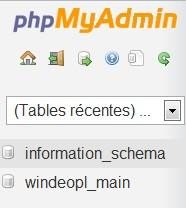
\includegraphics[scale=0.4]{images/6}
  \caption{Etape 6: choix du type de paiement}
\end{figure}

\newpage
\textbf{Etape 7: activeX paiement}\\

Si l’utilisateur choisi de payer via l’active X, la procédure est identique qu’à l’étape 3 mais il lui sera demandé un code PIN (voir étape 8) pour s’assurer qu’il est bien le porteur de la carte.
\begin{figure}[!htbp]
  \centering
    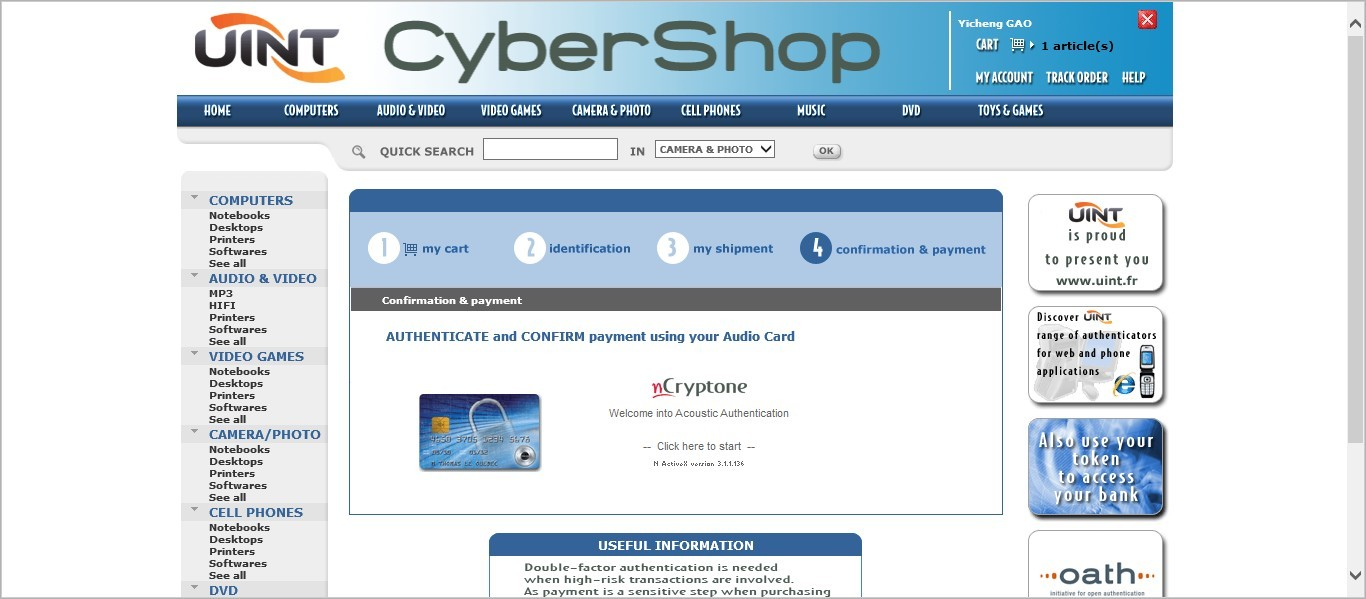
\includegraphics[scale=0.4]{images/7}
  \caption{Etape 7: activeX paiement}
\end{figure}
\vspace{2cm}

\textbf{Etape 8: demande du code pin}\\

Pour s’assurer que le porteur de la carte est bien celui qu’il prétend être, il lui est demandé un code PIN qu’il doit saisir à la souri ou au clavier.
La signature acoustique ainsi que le code pin sont envoyés de manière sécurisée au serveur d’authentification. Si les 2 informations sont correctes, l’utilisateur est alors redirigé vers la page lui confirmant son achat (étape 10)
\begin{figure}[!htbp]
  \centering
    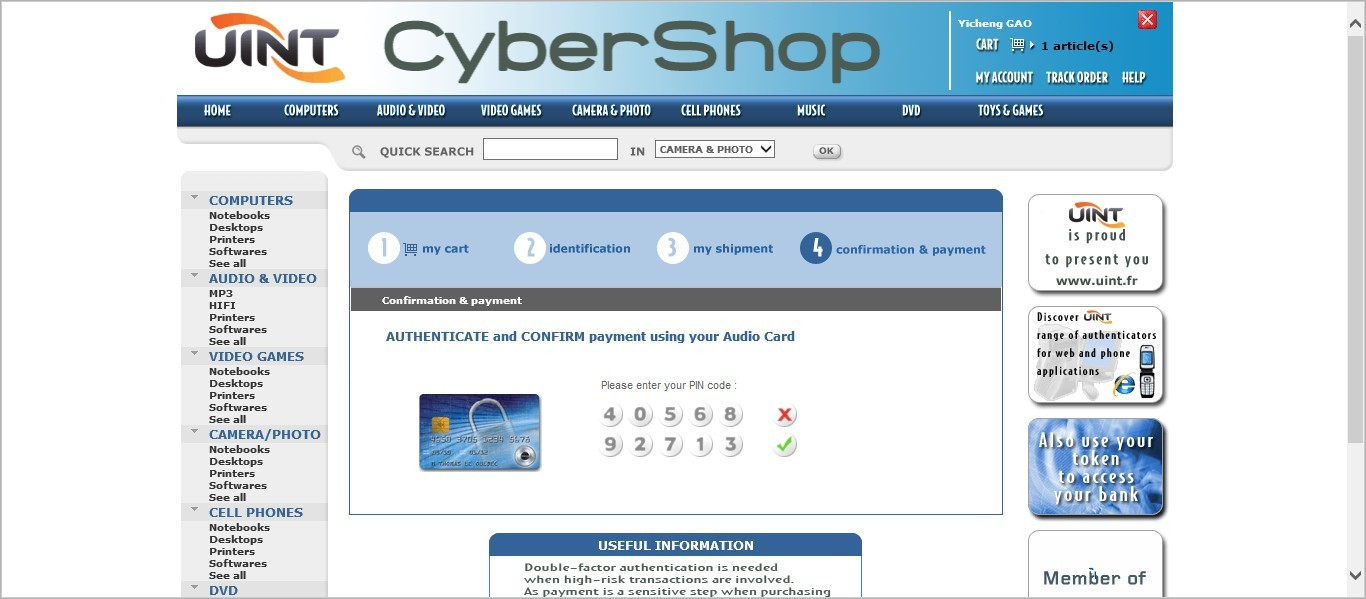
\includegraphics[scale=0.4]{images/8}
  \caption{Etape 8: demande du code pin}
\end{figure}

\newpage
\textbf{Etape 9: authentification par le serveur vocal}\\

Dans le cas où lors de la demande du type de paiement, l’utilisateur choisi l’option «serveur vocal», une fenêtre s’ouvre lui demandant d’appeler un numéro de téléphone pour se faire rappeler ou s’identifier directement.
Un numéro de session s’affiche dans la pop-up, il devra être retapé à l’aide du clavier de son téléphone. L’utilisateur devra ensuite utiliser sa carte contre le combiné de son téléphone, puis saisir son code PIN.
Les informations sont ensuite vérifiées par le serveur d’authentification. Si celles-ci sont correctes, l’utilisateur est automatiquement redirigé vers la page confirmant son achat (étape 10).
\begin{figure}[!htbp]
  \centering
    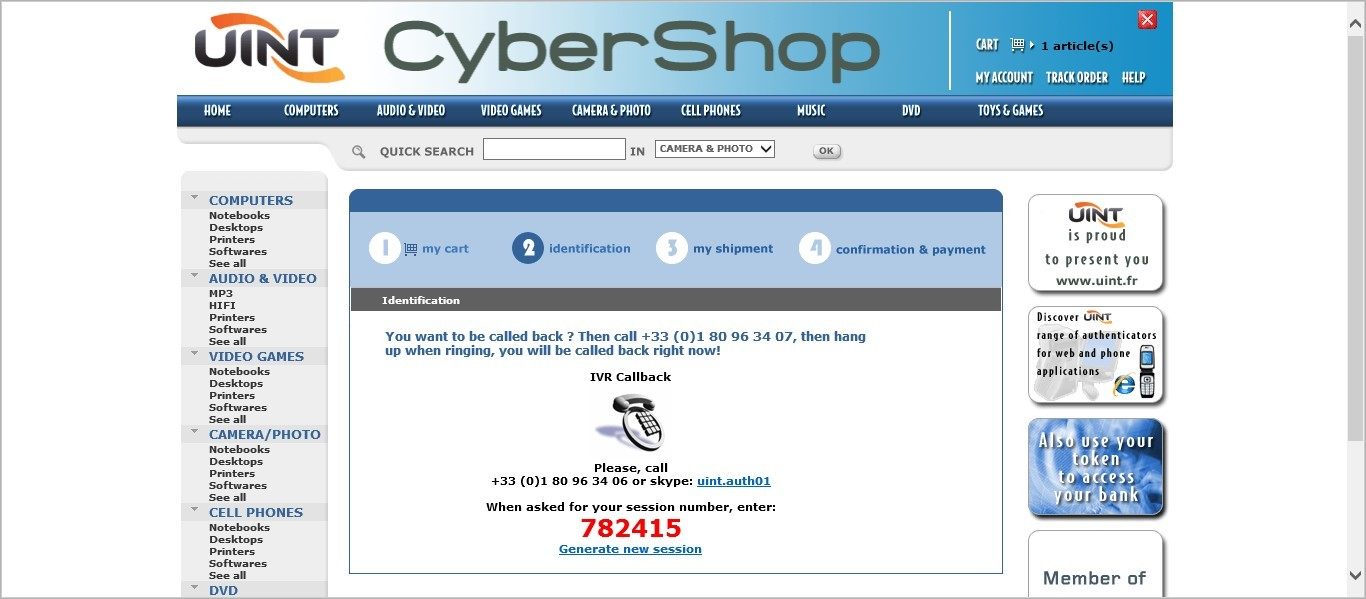
\includegraphics[scale=0.4]{images/9}
  \caption{Etape 9: authentification par le serveur vocal}
\end{figure}

\textbf{Etape 10: finalisation de l’achat}\\

Cette dernière étape est la confirmation de l’achat.
Un mail ainsi qu’un SMS sont envoyés à l’utilisateur lui indiquant les informations de son achat.
\begin{figure}[!htbp]
  \centering
    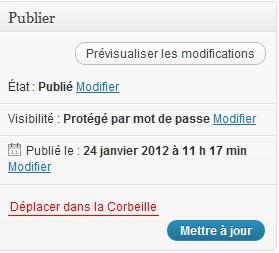
\includegraphics[scale=0.4]{images/10}
  \caption{Etape 10: finalisation de l’achat}
\end{figure}

%%%%%%%%%%%%%%%%%%%%%%%%%%%%%%%%%%%%%%%%%%%%%%%%%%%%%%%%%%%%%%%%%%%%%%%%%%%%%%%%%%%%%%%%%%%%%%%%%%%%%%%%%%%%%%%%%%%%%%%%%%%%%%%%%%%%%%%%%%%%
\newpage
\subsection{Principe de fonctionnement}

Cette démo d’un magasin de vente en ligne, repose sur 4 acteurs:
\begin{itemize}
\item L’utilisateur et sa carte
\item Le serveur Web
\item Le serveur d’authentification
\item Le serveur vocal
\end{itemize}

\begin{figure}[!htbp]
  \centering
  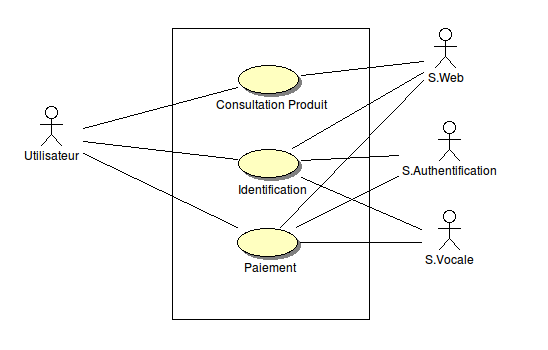
\includegraphics[scale=0.6]{images/uml1}
  \caption{Diagramme des cas d'utilisation} 
\end{figure}


\newpage
Voici un diagramme de séquence décrivant la procédure en utilisant le serveur vocale:

\begin{figure}[!htbp]
  \centering
  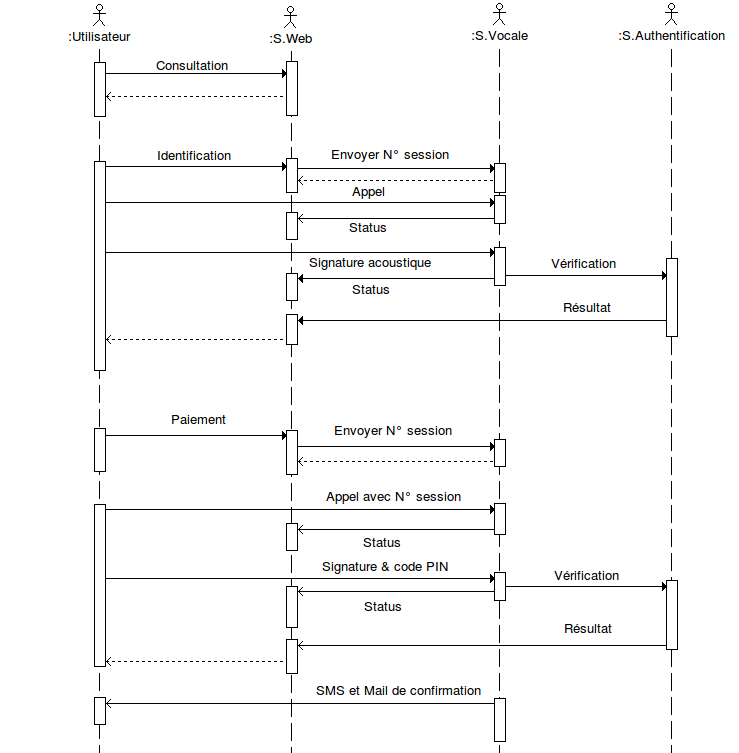
\includegraphics[scale=0.7]{images/uml2}
  \caption{Diagramme de séquence} 
\end{figure}

\newpage

%%%%%%%%%%%%%%%%%%%%%%%%%%%%%%%%%%%%%%%%%%%%%%%%%%%%%%%%%%%%%%%%%%%%%%%%%%%%%%%%%%%%%%%%%%%%%%%%%%%%%%%%%%%%%%%%%%%%%%%%%%%%%%%%%%%%%%%%
\subsection{Fonctionnement ActiveX}
% Voir le doc ActiveXIntgration.pdf pour plus d'information
\subsubsection{Présentation de l’ActiveX}

\begin{itemize}
\item[Dimension:]  237px $\times$ 96 px
\item[Couleur:] le fond est blanc et ne peut être changé
\item[Textes:] les textes sont modifiables directement dans le source de la page
\end{itemize}

\begin{figure}[!htbp]
  \centering
    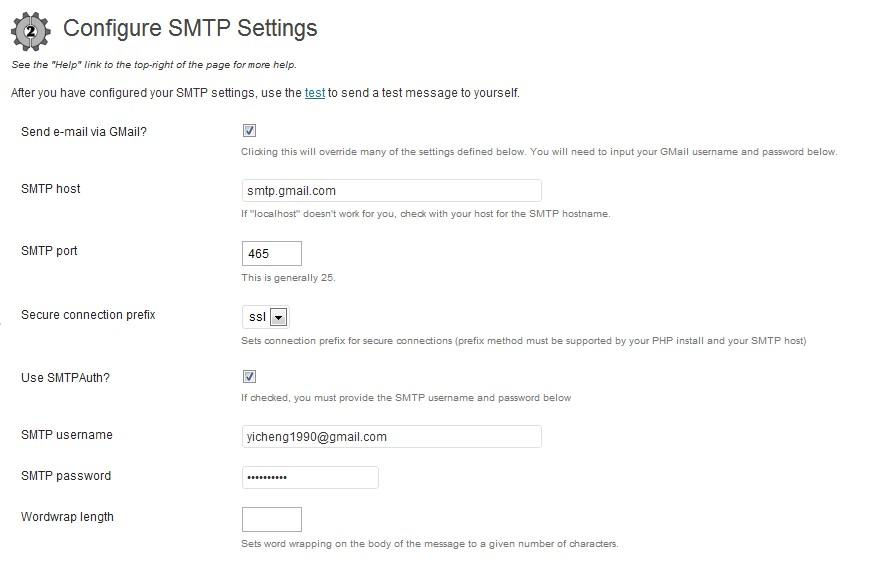
\includegraphics[scale=1.3]{images/11}
    \caption{L'affichage de l'ActiveX}
\end{figure}

\subsubsection{Initialisation de l’ActiveX}

L’ActiveX fonctionne dans 2 modes (tag nC\_vMode):\\

\indent \textbf{HTTP:} l’ActiveX transcode la signature acoustique reçue et forge un fichier xml codé contenant des informations relatives à la capture acoustique ainsi que son environnement\\
\indent \textbf{JAVASCRIPT:} l’ActiveX transcode la signature et la met à disposition d’une fonction javascript. Seul le message acoustique est transmis.\\

Suivant le contexte de l’intégration, on s’orientera vers l’un ou l’autre des 2 modes.\\

Dans le mode HTTP, l’ActiveX récupère le message acoustique émis par la carte, le formatte dans un fichier xml et l’envoi en POST à l’url indiquée par la valeur de l’input «nC\_vURL».\\

%%%%%%%%%%%%%%%%%%%%%%%%%
% À ajouter dans annexe %
%%%%%%%%%%%%%%%%%%%%%%%%%


Dans le mode JAVASCRIPT, à l’issu du transcodage, la signature acoustique est transmise à la fonctionJavascript «nC\_Authenticate».\\
%%%%%%%%%%%%%%%%%%%%%%%%%
% À ajouter dans annexe %
%%%%%%%%%%%%%%%%%%%%%%%%%


L’avantage du mode JAVASCRIPT est de permettre facilement la manipulation du numéro de série pour faire des traitements avant l’envoi au serveur d’authentification.\\

La présence de tous ces tags HTML dans le code d’une page permet l’affichage de l’ActiveX.\\
\newpage
L’utilisateur doit cliquer dans l’ActiveX pour initialiser la capture acoustique.\\

\begin{figure}[!htbp]
  \centering
    
\includegraphics[scale=1.3]{images/22}
    \caption{L'affichage si activée}
\end{figure}


Une fois la capture réalisée, l’ActiveX envoi les informations à la page spécifiée dans le tag HTML «nC\_vURL»

\subsubsection{Envoi des informations récupérées par l’activeX au serveur d’authentification}

Le traitement des fichiers XML et l’envoi d’une requête WEB peuvent être réalisés par n’importe quel framework.\\

Le serveur PHP va récupérer les informations envoyées par l’ActiveX et les soumettre au serveur d’authentification via les WebServices.

%%%%%%%%%%%%%%%%%%%%%%%%%%%%%%%%%%%%%%%%%%%%%%%%%%%%%%%%%%%%%%%%%%%%%%%%%%%%%%%%%%%%%%%%%%%%%%%%%%%%%%%%%%%%%%%%%%%%%%%%%%%%%%%%%%%%%%%%%%%%%
\newpage
\subsection{Fonctionnement serveur vocal}

\subsubsection{Scénario}
\begin{figure}[!htbp]
  \centering
    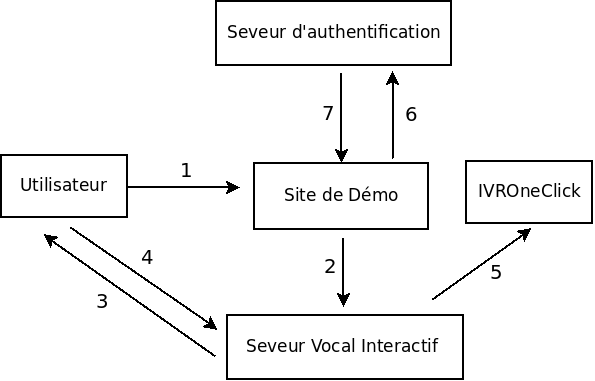
\includegraphics[scale=0.5]{images/Diagramme1}
\end{figure}

\begin{enumerate}
\item Après l'authentification. Le numéro de téléphone d'utilisateur est enregistré en base de données
\item Le serveur Web envoie une requête au serveur vocal interactif avec comme paramètres (numéro de session + numéro de téléphone + demande de code pin)
\item Le serveur vocal interactif rappelle l’utilisateur sur le numéro de téléphone renseigné
\item L’utilisateur utilise sa carte et son code pin (L'utilisateur peut aussi être demandé un code envoyé par SMS selon le mode de carte WEGA)
\item Le serveur vocal interactif envoie ces informations au serveur web. Le serveur web lui renvoie une réponse indiquant si les informations en base de données ont été mises à jour
\item Le serveur web réalise l’authentification avec les informations fournies et indique à l’utilisateur le résultat de l’authentification
\end{enumerate}


\subsubsection{Principe}
Le dialogue entre le SVI et le serveur web se fait à l’aide de 2 pages Web.
Ces 2 pages Web doivent donc être accessibles de l’extérieur (via un VPN par exemple) ou alors en local si les 2 serveurs sont sur le même réseau.\\
\begin{itemize}
\item Une première page permet au SVI de savoir si une session est valide ou pas et s’il doit demander un code Pin à l’utilisateur
\item La deuxième page permet au SVI d’envoyer au serveur web la signature acoustique de la carte et le code pin
\end{itemize}

\subsubsection{Numéro de session}
Lorsque l’utilisateur désire s’identifier via le serveur vocal, le serveur web doit créer un numéro de session de 6 chiffres, qu’il va mettre en base de données. S’il s’agit d’une authentification, le serveur web doit également indiquer dans la base de données qu’un code pin sera demandé. \\


\subsubsection{Exemple de présentation}

\begin{figure}[!htbp]
  \centering
    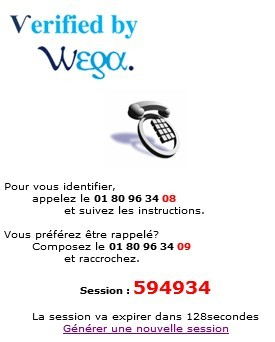
\includegraphics[scale=0.8]{images/33}
\end{figure}

\subsubsection{Exemple de la structure de la Base de Données}

\begin{center}
\begin{tabular}{|c|c|}
\hline
\cellcolor[gray]{.7}Nom du champ & \cellcolor[gray]{.7}Type\\ \hline
Session & varchar\\ \hline
DtStampInit & varchar\\ \hline
Status & int\\\hline
RAW & varchar\\ \hline
PINRequired & int\\ \hline
PINCode & varchar\\ \hline
DtStampSend & varchar\\ \hline
Demo\_Name & varchar\\ \hline
\end{tabular}
\end{center}


\subsubsection{GET\_Session}

Ce fichier est appelé par le SVI pour savoir si le numéro de session saisie par l’utilisateur sur son téléphone est valide ou pas. Un fichier XML est généré en retour à destination du SVI. Le serveur Web doit chercher dans sa base de données si le numéro de session reçu est valide ou pas.\\

\textbf{Input:}Session\\
Le SVI effectue via un POST à l’URL \texttt{http://<URL serveur web>/GET\_Session.php} avec comme paramètre «Session». Cette session contient les chiffres saisis par l’utilisateur sur le SVI.\\

\textbf{Output:}\\
Si une session a été trouvée dans la base de données, le fichier XML est alors retourné par le serveur web.

%\begin{lstlisting}
%<?xml version="1.0" encoding="ASCII" ?>; 
%<Result>
%<ExitCode>0</ExitCode>
%<ExitMessage>Session is OK</ExitMessage>
%<DtStampInit></DtStampInit>
%<PINRequired>1</PINRequired>
%</Result>
%\end{lstlisting}

\noindent L’attribut <ExitCode> est à 0 si la session a été trouvée, sinon il est à 1\\
L’attribut <ExitMessage> est la description du code erreur\\
L’attribut <PinRequired> est à 0 si le code Pin n’est pas requis, sinon il est à 1\\


%\textbf{Exemple d’intégration}

%%%%%%%%%%%%%%%%%%%%%%%%%
% À ajouter dans annexe %
%%%%%%%%%%%%%%%%%%%%%%%%%



\subsubsection{POST\_RAW}

Ce fichier permet au SVI de poster la signature acoustique de la carte ainsi que du code pin. Un fichier XML est généré pour indiquer au SVI si l’opération s’est bien déroulée.\\

Le serveur web reçoit plusieurs informations provenant du SVI via un POST à une URL précise du type \texttt{http://<URL serveur web>/POST\_RAW.php}, la session, le RAW (signature acoustique) et le code pin.\\

Le serveur doit mettre à jour sa base de données avec ces informations et retourner au SVI si l’opération s’est correctement déroulée.\\

\textbf{Input:}
\begin{itemize}
\item Session
\item RAW
\item PINCODE\\
\end{itemize}

\textbf{Output:} Fichier XML
\begin{lstlisting}
<?xml version="1.0" encoding="ASCII" ?>; 
<result>
<ExitCode>0</ExitCode>
<ExitMessage>Session is OK</ExitMessage>
</result>
\end{lstlisting}

 
%%%%%%%%%%%%%%%%%%%%%%%%%
% À ajouter dans annexe %
%%%%%%%%%%%%%%%%%%%%%%%%%

\subsubsection{Les paramètres}

Pour communiquer avec le serveur SVI, quelques paramètres sont nécessaires d'envoyer par POST ou GET selon le besoin. Il faut au moins le paramètre \textit{PhoneNumberToCall} pour émettre un appel (et \textit{SessionId} pour que le backoffice s’y retrouve après).\\

Les paramètres utilisés pour envoyer au SVI:\\

\noindent \textbf{PhoneNumberToCall:} est le numéro qui doit être appelé. Ce numéro doit être préférablement au format international sans le prefix\\
\textbf{DemoID:} permet d’identifier le serveur émetteur de la demande\\
\textbf{InternalPINCardRange1, InternalPINCardRange2:} sont des plages de numéros de série devant être gérée de façon particulière par le SVI\\
\textbf{SessionID:} est l’identifiant de session pour identifier de façon unique les demandes d’appels\\
\textbf{AskPIN:} valeur 0 ou 1 par défaut 0 indique au SVI s’il doit demander un code PIN après un détection carte\\

Dans la vitrine présentée dans le guide le SVI renvoi les résultat vers un serveur Web vitrine sous la forme d’un POST où sont les données précédentes ajoutées avec les information de carte PIN et les codes de statut de l’appel. \\

Il y a plusieurs status de l'appel:

\begin{center}
\begin{tabularx}{14.9cm}{|c|l|p{5cm}|}
\hline
Status Code&CONSTANT&Description\\ \hline
0&INIT&Initialisation\\ \hline
1&RAW\_RECEIVED&Signature acoustique transmise\\ \hline
2&CALL\_NOT\_ACCESSIBLE&Numéro inaccessible\\ \hline
4&INVALID\_PHONE\_NUMBER&Numéro invalide\\ \hline
8&CALL\_OCCUPIED&Ligne occupée\\ \hline
16&CALL\_NO\_ANSWERED&Pas de réponse\\ \hline
32&CALL\_REQUESTED&La demande de callback est reçue et prise en compte\\ \hline
33&CALL\_ANSWERED&L'appel est décroché\\ \hline
34&IVR\_CLOSE\_CALL&L'appel est raccroché\\ \hline
64&IVR\_ASK\_SEQ&L'IVR attend la séquence de la carte\\ \hline
65&IVR\_CARD\_NOT\_RECOGNIZED&Carte non reconnue\\ \hline
66&IVR\_ASK\_PIN&Attente saisie du code PIN\\ \hline
128&IVR\_CHECK\_RESULT&L'IVR envoie les informations de la séquence et attend la répense du serveur\\ \hline
256&INTERNAL\_ERROR&Erreur interne\\ \hline
\end{tabularx}
\end{center}

\subsubsection{Authentification}

Le serveur web doit donc vérifier si pour une session donnée, les informations de la capture acoustique et du code Pin sont présentes dans la base de données.\\

Le serveur web peut maintenant extraire ces informations de la base de données et réaliser une authentification ayant à sa disposition les informations de la carte et du code pin en utilisant les Web Services fournit par UINT.

%%%%%%%%%%%%%%%%%%%%%%%%%%%%%%%%%%%%%%%%%%%%%%%%%%%%%%%%%%%%%%%%%%%%%%%%%%%%%%%%%%%%%%%%%%%%%%%%%%%%%%%%%%%%%%%%%%%%%%%%%%%%%%%%%%%%%%%%%%%%%
\newpage
\subsection{SAS Web Services}
\label{SAS}
\subsubsection{Présentation générale}

Dans une première étape de tests et de validations UINT met à disposition un accès au SAS (Strong Authentication Server) pour valider des identités porteuses de cartes.\\

SAS fournit un certain nombre de services disponibles par Internet ou Intranet qui sera
permettre aux clients de:

\begin{itemize}
\item Vérifiez la disponibilité des serveurs
\item Récupérer des informations à partir de SAS
\item S'authentifier à l'aide d'un Token
\item Lister les informations d'identification des utilisateurs
\item Ajouter/Modifier les informations d'identification de l'utilisateur
\item Supprimer les informations d'identification d'un utilisateur
\item Récupérer les informations d'identification d'un utilisateur\\
\end{itemize}

Ces services Web peuvent être accessibles à partir de n'importe quel endroit à travers le protocole HTTP ou HTTPS.\\

\textbf{Modèle opération simple}\\
Les Webservices fournissent le modèle question-réponse d'une action ou demande d'information. Les échanges
entre SAS et demandeur de Webservices génère un identifiant de session qui peut être
jeté s'il n'est pas utilisé.\\

\textbf{Modèle Session}\\
Afin de manipuler des transactions complexes entre les Webservices et demandeur de services Web,
identification de session doit être géré sur les deux côtés offrent des fonctionnalités transactionnelles en particulier
des opérations de gestion.\\

\textbf{Formats}\\
La requête et les réponses peuvent être du texte, HTML ou XML.\\

\textbf{Demandes}\\
Une requête de Webservices peut être envoyer à SAS en utilisant la syntaxe de texte, de données ou en forme de chiffrement.\\

\textbf{Réponses}\\
Le SAS répond aux requêtes de Webservices avec le format requis définis dans la requête.\\

\textbf{Sessions}\\
Les requêtes et les réponses sont effectuées en utilisant la gestion des sessions SAS et fournissent caractéristiques transactionnels.

\subsubsection{Syntaxe}

Une requêtes WebServices doit suivre la syntaxe suivante:

\texttt{HTTP[S]://SASAddress[:Port]/WEBSERVICES?\\
\indent \indent \indent \indent \indent \indent \indent \indent OP=[OPERATION][\&PARAMETERVALUE=[Parameter Data]]}\\

Les paramètres optionnels:\\
\texttt{
\&INFORMAT=[Input Format]\\
\&OUTFORMAT=[Output Format]\\
\&SKEY=[Session Key]\\
\&DATA=[XMLData]\\}


\textbf{SASAddress}\\
C'est l'adresse SAS au format numérique comme 192.168.2.204 ou au format canonique comme
Authentication.UnipaysINTelligence.com\\

\textbf{Port}\\
Indique le port TCP que SAS écoute. La valeur par défaut, lorsqu'il n'est pas défini, est de 80 en utilisant le préfixe http
et le port 443 en utilisant https. \\

\textbf{/WEBSERVICES?OP=}\\
Indique quelle requêtes de WebServices sera traitée par le SAS.\\

\textbf{OPERATION}\\
Le type d'opération que SAS à effectuer.


Pour simplifier avec les Web Services, iL y a trois commandes à considérer:
\begin{itemize}
\item \textit{ISALIVE} pour vérifier que le serveur est online, pourrait être ignorée mais signifie de gérer un timeout sur la commande suivante.
\item \textit{AUTHTOKEN} pour tester le message d’authentification
\item \textit{LOGOUT} pour fermer la session avec le serveur.
\end{itemize}

Les codes retour à considérer sont :
\begin{itemize}
\item Pas de communication avec le serveur suite à la command \textit{ISALIVE}
\item Echec authentification suite à la commande \textit{AUTHTOKEN}
\item Réussite authentification suite à la commande \textit{AUTHTOKEN}
\end{itemize}


\subsubsection{Exemples d'utilisation}
\newpage
\textbf{Exemple 1: Exemple de service Web simple renvoyant une sortie type XML}\\

Cet exemple permet de récupérer les informations générales SAS et le statut avec la sortie type XML:\\

\noindent \textbf{REQUEST}\\
\texttt{http://Authentication.UnipaysINTelligence.com/WEBSERVICES?OP=\\
ISALIVE\&OUTFORMAT=512}\\
\textbf{RESULTAT}
\begin{lstlisting}
<?xml version="1.0" encoding="ASCII"?>
<Data>
<ServerInfo>
  <Session>
    <SessionID>8157e499-7766-4d9c-9013-9880c8280b72</SessionID>
  </Session>
  <Identity>
    <Version>3.0.278</Version>
    <ServerName>SSPRO</ServerName>
    <SID>AA</SID>
    <PublicKey>0602000000a40000525341310002000001000100f5c51d9cc8
    a78a9b7e221128a70eb7110016a8b7d4f7842c2998dc9b36f3f654c9b48aa
    4bdb56bd406640dae89782bd7bdf25cd45da6cc162c5233605e2634a8</PublicKey>
  </Identity>
  <Localization>
    <TimeZone>2</TimeZone>
    <LocalTime>20040803195315</LocalTime>
    <UTCTime>20040803175315</UTCTime>
    <Country>France</Country>
    <CountryIndex>64</CountryIndex>
  </Localization>
  </ServerInfo>
  <result>
    <ExitCode>0</ExitCode>
    <ExitMessage/>
  </result>
</Data>
\end{lstlisting}

\vspace{2cm}
\textbf{Exemple 2: Exemple de service Web simple renvoyant une sortie type HTML}\\

\noindent \textbf{REQUEST}\\
\texttt{http://Authentication.UnipaysINTelligence.com/WEBSERVICES?OP=\\
ISALIVE\&OUTFORMAT=256}\\
\textbf{RESULTAT}\\
\texttt{OK}\\



% ------------- CONCLUSION -------------- %

\section{Conclusion}
\begin{frame}
\frametitle{Conclusion}
	\begin{block}{Les r�alisations}
		\begin{itemize}
		\item Plate-forme de tests: Les r�sultats sont bien pris en compte
		\item Plate-forme de d�monstration: L'application web est enti�rement fonctionnelle
		\end{itemize}
	\end{block}

	\begin{exampleblock}{Bilan personnel}
		\begin{itemize}
		\item Dur�e
		\item Mettre en oeuvre autour des trois fili�res ASI
		\begin{itemize}
			\item Acquisition de l'information
			\item Traitement de l'information
			\item Informatique
		\end{itemize}
		\item Jouer des r�les multiples 
		\end{itemize}
	\end{exampleblock}

\end{frame}


% ---------------------------------------- %
\begin{frame}
	\frametitle{Fin de la pr�sentation}
	\begin{figure}
	
\includegraphics[scale = 0.45]{images/question.jpg}	
	\end{figure}
	
	\begin{center}
	\textbf{Merci de votre attention}
	\end{center}

\end{frame}
\end{document}
